\chapter{基于锁的并发数据结构}
\thispagestyle{empty}

%\section{引言}
在结束锁的相关内容之前,先讲一讲在一些常用的数据结构中怎么使用锁。在数据结构中添加锁能够让此结构体线程安全(thread safe),这对线程是很有用的。当然,确切地讲锁的添加方式决定了该数据结构的正确性和性能。因此,面临的挑战:

\begin{tcolorbox}[colframe=grey,colback= grey,arc=0pt,left=6pt,right=6pt,top=6pt,bottom=6pt,boxsep=0pt]
\begin{center}Crux:如何将锁添加到数据结构中\end{center}
给定一个特定的数据结构时,该如何把锁加进去使之可以正确工作呢?进一步,如何使添加了锁的数据结构实现高性能,让多线程可以立即访问到该数据结构,比如并发地(concurrently)?
\end{tcolorbox}

当然,由于这个话题已经研究了很多年了,已经发表了数千篇关于这个话题的论文,因此我们会尽力在本章中涵盖所有的数据结构或所有添加并发性性质的方法。因此,我们希望能为这些需要的想法提供足够多的介绍,以及给出一些好资源为你自己进一步学习提供帮助。Mior和Shavit的综述是一个很好的信息来源[MS04]。

\section{并发计数器}
最简单的数据结构是计数器。此数据结构经常使用且接口也简单。我们在图29.1中定义了一个简单的非并发计数器。

\begin{figure}[h]
\begin{lstlisting}
typedef struct __counter_t {
    int value;
} counter_t;

void init(counter_t *c) { 
    c->value = 0;
}
    
void increment(counter_t *c) {
    c->value++;
}

void decrement(counter_t *c) {
    c->value--;
}

int get(counter_t *c) { 
    return c->value;
}
\end{lstlisting}
\caption{不使用锁的计数器}
\end{figure}

\textbf{简单但不可扩展}


\begin{verbatim}
\end{verbatim}

正如你所看到的,无同步的计数器是一个很平凡的数据结构,只需很少的代码即可实现。那问题来了:怎么使之线程安全(thread safe)?图29.2展示了我们是怎么做的。
\begin{figure}[h]
\begin{lstlisting}
typedef struct __counter_t {
int value;
pthread_lock_t lock;
} counter_t;

void init(counter_t *c) {
c->value = 0;
Pthread_mutex_init(&c->lock, NULL);
}

void increment(counter_t *c) {
Pthread_mutex_lock(&c->lock);
c->value++;
Pthread_mutex_unlock(&c->lock);
}

void decrement(counter_t *c) {
Pthread_mutex_lock(&c->lock);
c->value--;
Pthread_mutex_unlock(&c->lock);
}

int get(counter_t *c) {
Pthread_mutex_lock(&c->lock);
int rc = c->value;
Pthread_mutex_unlock(&c->lock);
return rc;
}
\end{lstlisting}
\caption{使用锁的计数器}
\end{figure}

\begin{figure}[h]
\begin{lstlisting}

\end{lstlisting}
\caption{}
\end{figure}

这个并发计数器简单有效。实际上,它遵循了常见的最简单也最基本的并发数据结构设计模式:简单地加一个锁,即在操作该数据结构时上锁,在返回时解锁。这种方法与用monitors[BH73]构造的数据结构类似,在你调用该对象的接口和从该接口返回时自动的上锁以及解锁。

此时,你就有了一个可以用的并发数据结构。可能你会关心的是它的性能。要是数据结构性能太低,那你就不仅仅是加一个锁了;如果需要的话,还要优化,这也是接下来本章将要讨论的。记住,如果数据结构的性能可以的话,那就OK了!简单可行的东西就没有必要再做一些花里胡哨的事儿。

为了弄明白这个简单方法的性能开销,我运行一个benchmark,这个benchmark中每个线程共同更新一个共享计数器固定次数;然后改变线程数。图29.3是时间开销,分别是1-4个线程;每个线程更新计数器百万次。这个实验运行在一台iMac上,4个Intel 2.7GHz i5CPU;要是有更多的CPU,我们希望单位时间内能完成更多的工作。

\begin{figure}[h]
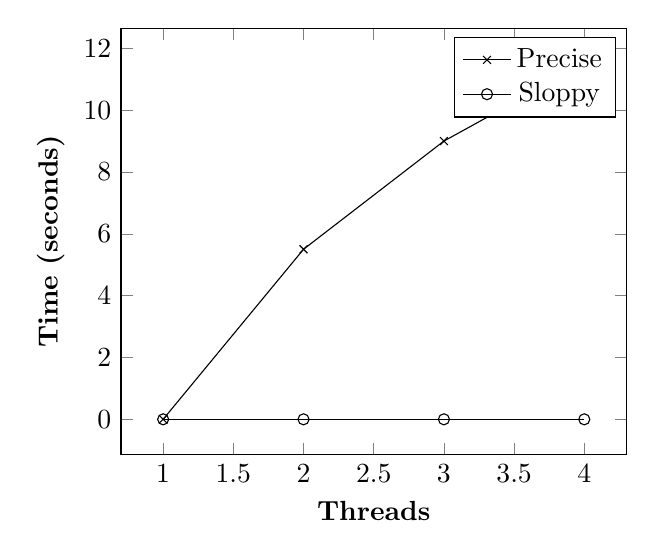
\begin{tikzpicture}
    \begin{axis}[
        ylabel=\textbf{Time (seconds)},
        xlabel=\textbf{Threads},
        width = 8cm,
        height= 7cm
    ]
    \addplot[black,mark=x] plot coordinates {
        (1,    0)
        (2,   5.5)
        (3,   9)
        (4,   11.5)
    };

    \addplot[black,mark=o] plot coordinates {
        (1,   0)
        (2,   0)
        (3,   0)
        (4,   0)
    };

    \legend{Precise\\Sloppy\\}
    \end{axis}
\end{tikzpicture}
\caption{traditional vs. sloppy计数器的性能}
\end{figure}

从图中上面的一条线(precise标记),可以看出同步计数器的性能扩展很差。然而单线程可以在很短的时间内完成百万次的计数器更新(0.03秒),当两个线程各自并发地更新计数器百万次时,性能就急剧下降(超过5秒)。线程数更多则结果越差。

理想情况下,希望看到运行在多处理器上的多线程如单处理器单线程一样快。实现这一目标的话,那就是完美扩展(perfect scaling)了;即使已经有了很多研究工作,但它是以并行方式完成的,因此完成此项任务的时间并没有增加。


\textbf{可扩展计数}
令人惊讶的是,研究人员就如何构建具有更好扩展性的计数器已经研究了很多年[MS04]。更令人惊喜的是可扩展计数器很重要这一事实,正如[B+10]最近在操作系统性能分析方面的工作表明的;如果没有可扩展计数器,某些多核机器上的Linux负载就会有严重的扩展性问题。

已经开发了很多技术来解决这个问题,此处我们介绍其中一个方法。其思想由最近的一篇论文[B+10]提出,即sloppy counter。

sloppy counter通过多个局部物理计数器代表一个全局逻辑计数器,每个核都有一个局部物理计数器。具体的,一个4CPU的机器,有四个局部计数器和一个全局计数器。除这些计数器外,还有锁:每个局部计数器和全局计数器各自都有一个锁。

sloppy counter的基本思想如下。当运行在某个核上的某个线程想要加计数器时,它就增加该核的局部计数器;通过对应的局部锁访问这个同步局部计数器。由于每个CPU都有自己的局部计数器,多CPU上的多线程就可以无竞争地更新局部计数器,因此计数器的更新是可扩展的。

然而,为了保持全局计数器保持最新(万一某个线程想要获取这个值呢),局部值会定期提交给全局计数器,通过获取全局锁访问全局计数器并加之以局部计数器的值;然后局部计数器的值重置为0。

局部到全局的更新多久提交一次是由一个门限值决定的,这里称门限值为S(soppiness)。S值越小,就与不可扩展计数器类似;S值越大,该计数器扩展性就越好,但是全局计数器的值就会与真实值差别越大。可以简单的获取所有的局部锁和全局锁(以某一特定顺序,以防死锁)来得到准确值,但这是不可扩展的。

为了更清晰的理解这个问题,来看一个例子(表29.1)。这个例子里,门限值设为5,4个CPU上各自有一个线程更新其局部计数器L1 … L4。全局计数器的值(G)也显示在表中,之间自上向下增长。每一步中,局部计数器都有可能会增长;如果局部计数器达到了门限值,局部计数器值就会提交给全局计数器并重置为0。
\begin{figure}[h]

\caption{}
\end{figure}
表29.1

图29.3中下面的一条线显示sloppy counter在门限值S为1024时的性能。其性能非常的好;在四个处理器上更新计数器四百万次的时间与单处理器上更新百万次的时间相比几乎不多多少。

图29.5显示了门限值S的重要性,此图为四个线程在四个CPU上各自更新计数器百万次。如果S太低,性能很差(但是全局值会比较精确);如果S很高,性能就会很好,但是全局值会有延迟(决定于CPU个数*S)。精确度与性能之间的权衡是sloppy counter要考虑的。

\begin{figure}[h]

\caption{}
\end{figure}
图29.5

一个粗略的sloppy counter代码见图29.4。看一看,自己写一遍的话更好,这样可以更好的理解它是怎么运行的。


\begin{figure}[h]
\begin{lstlisting}
typedef struct __counter_t {
int global; // global count
pthread_mutex_t glock; // global lock
int local[NUMCPUS]; // local count (per cpu)
pthread_mutex_t llock[NUMCPUS]; // ... and locks
int threshold; // update frequency
} counter_t;

// init: record threshold, init locks, init values
// of all local counts and global count
void init(counter_t *c, int threshold) {
c->threshold = threshold;

c->global = 0;
pthread_mutex_init(&c->glock, NULL);

int i;
for (i = 0; i < NUMCPUS; i++) {
c->local[i] = 0;
pthread_mutex_init(&c->llock[i], NULL);
}
}

// update: usually, just grab local lock and update local amount
// once local count has risen by ’threshold’, grab global
// lock and transfer local values to it
void update(counter_t *c, int threadID, int amt) {
pthread_mutex_lock(&c->llock[threadID]);
c->local[threadID] += amt; // assumes amt > 0
if (c->local[threadID] >= c->threshold) { // transfer to global
pthread_mutex_lock(&c->glock);
c->global += c->local[threadID];
pthread_mutex_unlock(&c->glock);
c->local[threadID] = 0;
}
pthread_mutex_unlock(&c->llock[threadID]);
}

// get: just return global amount (which may not be perfect)
int get(counter_t *c) {
pthread_mutex_lock(&c->glock);
int val = c->global;
pthread_mutex_unlock(&c->glock);
return val; // only approximate!
}
\end{lstlisting}
\caption{}
\end{figure}
图29.4


\section{并发链表}
下面讲一个稍微复杂已点的数据结构:链表。这次也先从基本的方法开始。简单起见,我们会省略一些显而易见的代码,并重点关注并发插入;把查询、删除等留给读者思考。图29.6展示了这一基础数据结构的代码。

\begin{figure}[h]
\begin{lstlisting}
// basic node structure
typedef struct __node_t {
int key;
struct __node_t *next;
} node_t;

// basic list structure (one used per list)
typedef struct __list_t {
node_t *head;
pthread_mutex_t lock;
} list_t;

void List_Init(list_t *L) {
L->head = NULL;
pthread_mutex_init(&L->lock, NULL);
}

int List_Insert(list_t *L, int key) {
pthread_mutex_lock(&L->lock);
node_t *new = malloc(sizeof(node_t));
if (new == NULL) {
perror("malloc");
pthread_mutex_unlock(&L->lock);
return -1; // fail
}
new->key = key;
new->next = L->head;
L->head = new;
pthread_mutex_unlock(&L->lock);
return 0; // success
}

int List_Lookup(list_t *L, int key) {
pthread_mutex_lock(&L->lock);
node_t *curr = L->head;
while (curr) {
if (curr->key == key) {
pthread_mutex_unlock(&L->lock);
return 0; // success
}
curr = curr->next;
}
pthread_mutex_unlock(&L->lock);
return -1; // failure
}
\end{lstlisting}
\caption{}
\end{figure}
图29.6

正如图中所示,该代码简单的在插入函数入口获取锁,在退出时释放锁。如果malloc()碰巧失败的话(极少情况下),这个问题就会很棘手;这种情况下,仍然必须在插入失败之前释放锁。

这种异常控制流程已被证明是相当容易出错的;最近的Linux内核补丁研究发现相当一部分(接近四成)的bug是由于这个很少采用的控制流程造成的(确实,这个研究结果激发了我们自己的研究,我们从一个Linux文件系统移除了所有的内存失败分支,从而得到了一个更健壮的系统[S+11])。

因此,挑战:上述的失败分支中仍然需要调用unlock,我们是否可以在避免它的情况下,重写插入和查询函数以保证并发插入时仍保持正确性?

这种情况的答案是yes。具体说,我们可以稍微重新组织一下代码,让加锁和解锁仅仅出现在插入函数中真正的临界区周围(译者注:即尽量缩小临界区的大小),这样共同的退出路径也用在查询函数中。前者可行是因为查询的部分代码实际上不需要加锁;假设malloc()自身是线程安全的,每个线程都可以调用而不用担心竞争条件或者其他的并发问题。只有当更新共享链表时才需要加锁。修改后的代码详见图29.7。

\begin{figure}[h]
\begin{lstlisting}

\end{lstlisting}
\caption{}
\end{figure}
图29.7

关于lookup函数,就是简单的变换一下 ,跳出住循环至同一个单独的返回路径。这样做可以降低代码中锁的获取释放点的数量,因此降低了意外地引入bug的几率(比如忘记在返回前解锁)。

\textbf{扩展链表}
尽管又得到了一个基本的并发链表,但是我们又要问自己:具体哪儿的扩展性不好?研究人员开发出一个可以使链表并发性提高的技术:hand-over-hand locking(即:锁耦合)[MS04]。

上述技术的思想很简单。并非整个链表拥有一个锁,而是每个节点各自拥有一个锁。当遍历这个链表时,需要先获取下一个节点的锁在释放当前节点的锁(这不就像手牵手嘛)。

从概念上讲,这种链表是有一定意义的;它使得链表操作有了高度的并发性。然而,实际上,要让这样的链表运行的比简单方法快还是很很难的,因为在一次链表遍历中获取、释放每个节点锁的开销还是很大的。即便是非常大的链表以及大量的线程,这种方法的并发性也不太可能比简单方法的并发性高。也许某种混合方法(即多个节点一个锁)值得调研一下。

TIP:更高的并发性并不一定更快
如果你设计的方案增加了大量的负载(比如频繁地加锁解锁操作),更高并发性也许并不重要。如果开销高的函数使用的不多的话,简单的方法可能更好。增加更多的锁和复杂性可能会使性能下降。说这么多,有一个方法可以知道哪种更好:构建两个可选方案,并各自测量一下。性能是不会欺骗人的,这样就可以知道你的想法是否更快。

TIP:提防锁和控制流程
这里有一个在开发并发程序时很有用的通用设计建议:小心控制流的改变,比如会导致函数返回、退出或其他类似的会停止函数执行的错误条件。因为很多函数开始会加锁、分配一些内存或者其他一些类似的有状态的操作,当发生错误时,需要在返回前取消这些状态,否则会出错。因此,最好将代码条理化以最小话出错的概率。


\section{并发队列}
正如你所看到的,有一个标准的方法来构造一个并发数据结构:增加一个大锁。对于队列,我们就跳过这一部分,认为你自己能够弄明白它。

相反,我们会看一个并发性稍有提升的并发队列,由Michael和Scott设计[MS98]。此数据结构及其相关代码见图29.8。

\begin{figure}[h]
\begin{lstlisting}

\end{lstlisting}
\caption{}
\end{figure}
图29.8


如果你仔细研究这段代码的话,你会发现这里有两个锁,一个在锁队首,一个在队尾。这么做的目的是使得入队与出队操作能够并发操作。通常,入队函数仅访问队尾的锁,出队仅访问队首的锁。

Michael和Scott用了个技巧,他们在队列初始化时分配了一个dummy节点;这个节点将队首和队尾操作分割开了。好好研究这段代码,最好自己写一遍、运行并测量一下,这样才能更深入的理解它是如何运作的。

队列经常用在多线程应用中。然而,这里讲的队列类型通常不能完全适应该程序的需求。一个开发的更完整的有界队列是下一章——条件变量中将要认真研究的主题,该队列会使得线程在队列空或满时等待。


\section{并发哈希表}
最后一个要讨论的是简单但广泛应用的并发数据结构:哈希表。我们重点关注大小不变的简单Hash表;要处理改变大小的话,还需要一些额外的工作,这部分就留给读者当做练习。

此处的并发哈希表很简单,直接用早前开发的并发链表来构造,用起来还挺好。能有如此良好性能的原因是每个哈希bucket都有一个锁(即每个lists成员都有一个锁),而不是一整个数据结构只有一个锁。这样就可以同时发生多个并发操作。

\begin{figure}[h]
\begin{lstlisting}
#define BUCKETS (101)

typedef struct __hash_t {
list_t lists[BUCKETS];
} hash_t;

void Hash_Init(hash_t *H) {
int i;
for (i = 0; i < BUCKETS; i++) {
List_Init(&H->lists[i]);
}
}

int Hash_Insert(hash_t *H, int key) {
int bucket = key % BUCKETS;
return List_Insert(&H->lists[bucket], key);
}

int Hash_Lookup(hash_t *H, int key) {
int bucket = key % BUCKETS;
return List_Lookup(&H->lists[bucket], key);
}
\end{lstlisting}
\caption{}
\end{figure}

图29.10显示了哈希表并发更新的性能(4个线程各自执行1万到5万次并发更新,在相同的4CPU的iMac上)。作为对比,还显示了只使用一个锁的链表的性能。从图中可以看到,简单的并发哈希表的扩展性非常好;相反,链表却很差。

\begin{figure}[h]

\caption{}
\end{figure}
图29.10

TIP:不要过早优化(Knuth定律)
当构建一个并发数据结构时,先从最基本的方法开始,即增加一个大锁实现同步访问。这么做,可以先构造一个正确的的结构;然后,如果发现存在性能问题,再改进它。因此,仅仅在需要的时候为其提速。如Knuth的名言:”过早优化是万恶之源。“
许多操作系统在过度到多处理器时都是增加一个锁,包括Sun OS和Linux。后来,甚至起了个名字:大内核锁(big kernel lock,BLK),这也是多年来性能问题源头,直到2011年才消除了影响。在SunOS中(BSD的变种),移除保护内核的大内核锁非常痛苦,故而Sun工程师们决定另起炉灶:构造一个全新的Solaris操作系统,因此Solaris一开始就是多线程操作系统。可以阅读Linux和Solaris内核书籍获得更多的信息[BC05,MM00]。


\section{小结}
已经介绍了一些并发数据结构的样例,从计数器到链表和队列,最后是无所不在的哈希表。这一路过来,我们已经学了很多:在控制流改变时小心的获取、释放锁;过多的并发性不一定能提升性能;只有真正有性能问题时才需要去解决。最后一点——过早优化,对于很多关心性能的开发者来说是核心;如果某一部分的速度提升无助于应用总体性能的提升,那是没有意义的。

当然,我们仅仅摸到了高性能数据结构的皮毛而已。可以看看Moir和Shavit非常号的综述以获得更多信息,以及其他资源的链接[MS04]。特别的,你也许对其他数据结构也感兴趣(比如B树);数据库类库使你最好的选择。也许你也对那些不用传统锁的技术;比如非阻塞数据结构(non-blocking data structures),我们会在常见并发性bug那章中略作讲解,但坦白讲,这个话题需要更多的研究的领域,而这本入门书不太可能深入讲解。如果感兴趣的话,就自己去探索吧!

